\section{Indledning og Systembeskrivelse}

Sensorsystemer I tøj, ure, telefoner, belysning og mange andre hverdagsting bliver mere og mere populære. Dette projekt bruges som 
legeplads til at interface forskellige sensor systemer ved brug af et indlejeret system. Målet er at kunne gøre brug af projektets 
resultater i fremtidig systemudvikling. Den speciifikke case der behandles i dette system er et system der består af et GSM modem, 
en GPS reciever\footnote{GPS modtageren er ikke medtaget i det endelige projekt, slevom det i starten var tiltænkt} samt sensorer der kan måle temperatur, 
højder og barometrisk tryk. Data kan forespørges ved at sende en SMS der indeholder et sæt kommandoer.

Dette system er udviklet til at hente data fra en sensorer. Dette gøres ved at sende en sms til et telefonnummer, hvorefter der 
sendes et svar tilbage mede en måling fra den ønskede sensor.\\

På figur~\ref{fig:blockdiagram} ses et blokdiagram for systemet. Her på kan systemet største dele ses og hvordan disse kommunikerer. 
En nærmere beskrivelse af diverse komponenter findes i sektion~\ref{sec:blockdescription} på side~\pageref{sec:blockdescription}.

\vskip 0.5cm
\begin{figure}[h]
	\centering
	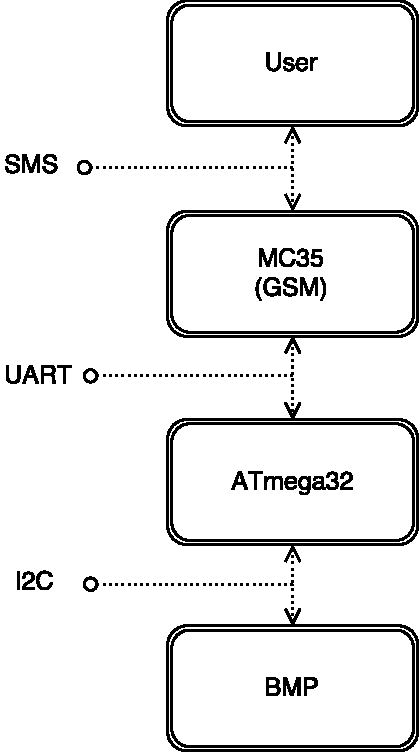
\includegraphics[width=\linewidth]{figs/blockdiagram.pdf}
	\caption{Blokdiagram for system.}
	\label{fig:blockdiagram}
\end{figure}
\vskip 0.5cm

Sekvensdiagrammet, figur~\ref{fig:seq-getdata} viser det overordnede flow igennem programmet fra at en bruger har sendt en sms, til at samme bruger får den ønskede måling tilbage.

\begin{figure}[h]
	\centering
	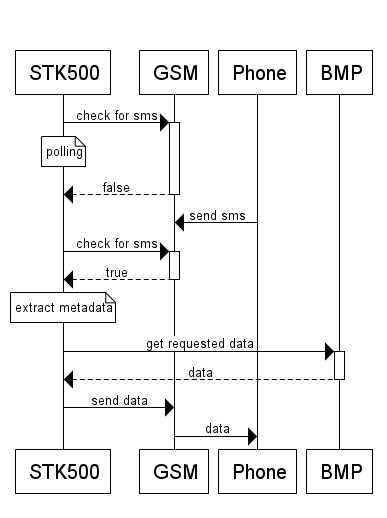
\includegraphics[width=0.56\linewidth]{figs/seq-getdata.png}
	\caption{Sekvensdiagram for anmodning og aflevering af data.}
	\label{fig:seq-getdata}
\end{figure}

\subsection{Valg af Sensor}
I dette projekt er der valgt en BMP085 sensor fra BOSCH, der er samlet på et lille breakout. Denne sensor er valgt, da den leverer tilstrækkelig høj målepræcision, og 
kan interfaces med I2C.
